% Perspective Projection Notes
\documentclass[11pt]{report}

\usepackage{amsmath}
\usepackage{amsfonts}
\usepackage{hyperref}
\usepackage{graphicx,color,geometry}
\usepackage{subcaption}

\begin{document}
	\title{\textbf{Notes on Perspecitve Projection Model for Shape from Shading}}
	\author{Balaje K, Sanath Keshav}
	\date{\today}
	\maketitle
	
	\pagebreak
	
	\section{Model Description}
	The Perspective Model assumes that the camera produces a perspective view of the scene on the screen as shown in Figure (\ref{fig:1}), as opposed to the orthographic projection model. Let us assume that the light source be placed at the focus/optical center of the camera.
	\begin{figure}[h!]
		\centering
		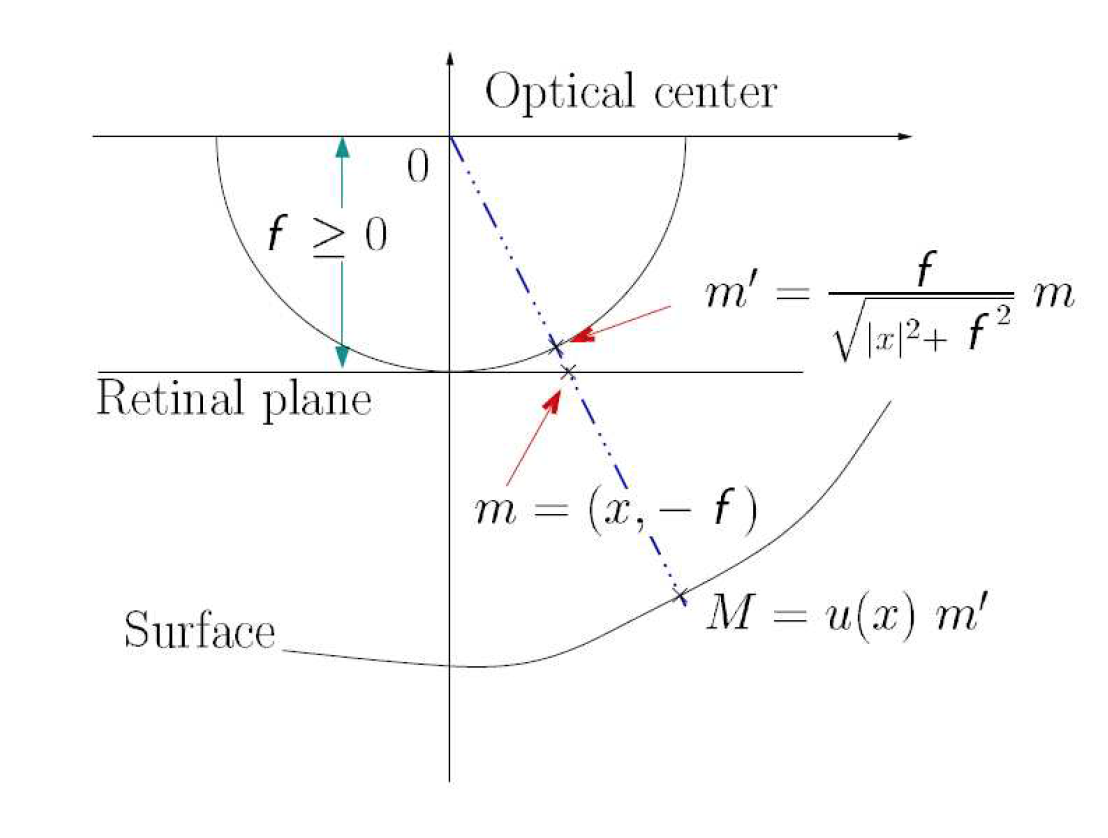
\includegraphics[scale=0.5]{focus.png}
		\caption{Perspective Projection with the light source at the focus}
		\label{fig:1}
	\end{figure}
	\noindent
	\\
	The surface can then be parametrized by,
	\begin{equation}
		\mathbb{S} = \left\{ \frac{f}{\sqrt{|\vec{x}|^2+f^2}}u(x_1,x_2)
		\begin{bmatrix}
		x_1\\
		x_2\\
		-f
		\end{bmatrix}
		\Bigg | (x_1,x_2)^T \in \bar{\Omega}
		\right\} \subset \mathbb{R}^3
	\end{equation}
	\\
	Using the brightness equation
	\begin{equation}
		I(\vec{x}) = \frac{\vec{L}}{|\vec{L}|} . \frac{\vec{n}}{|\vec{n}|}
	\end{equation}
	 \\
	 where $\vec{L} = \frac{1}{\sqrt{|\vec{x}|^2+f^2}}\begin{bmatrix}
	 x_1\\
	 x_2\\
	 -f
	 \end{bmatrix}$ is the Light vector and $\vec{n} = \mathbb{S}_{x_1} \times \mathbb{S}_{x_2}$ is the normal vector to the surface $z=u(x,y)$. Making all the necessary calculations, we arrive at a \textbf{Hamilton Jacobi Equation} with $v = \ln u$. This can be solved by appropriate boundary conditions.
	 \begin{equation}
	 	I(\vec{x})\sqrt{f^2|\nabla v|^2 + (\nabla v. \vec{x})^2 + \frac{f^2}{|\vec{x}|^2+f^2}} - \frac{f}{\sqrt{|\vec{x}|^2+f^2}} = 0 \label{eq:1}
	 \end{equation}
	 \\
	 The Hamiltonian $H(x,p) = I(\vec{x})\sqrt{f^2|p|^2 + (p. \vec{x})^2 + \frac{f^2}{|\vec{x}|^2+f^2}} - \frac{f}{\sqrt{|\vec{x}|^2+f^2}}$ can be shown that it is a convex function with respect to $p$. So we are in search of a viscosity sub-solution to the problem. Existence of the solution to the problem is guaranteed as long as,
	 \begin{equation}
	 	0 < I(\vec{x}) < 1
	 \end{equation}
	 and uniqueness is lost when $I(\vec{x})$ becomes equal to $1$, as the subsolution criterion becomes automatically invalid. In such cases, we are bound to \textit{supply the information} at those points. Naming these points as \textbf{singular points} and the set containing the points, as 
	 \begin{equation}
		 S = \{x\in\Omega , I(x) = 1\}
	 \end{equation}
	 we reformulate the boundary value problem as,
	 \begin{eqnarray}
	 	H(x,p) &=& 0 \;\;\; \text{in} \;\;\; \Omega - S = {\Omega}' \\
	 	u(x) &=& \phi(x) \;\;\; \text{on} \;\;\; \partial \Omega \cup S = \partial \Omega'
	 \end{eqnarray}
	 
	 \section{Numerical Scheme}
	 In this section, we develop a convergent numerical scheme to solve the \textbf{Hamilton Jacobi Equation} given by \ref{eq:1}. Rewriting the PDE by introducing a transient term $v_t$ to it, we have
	 	\begin{gather}
		v_t + I(\vec{x})\sqrt{f^2|\nabla v|^2 + (\nabla v. \vec{x})^2 + \frac{f^2}{|\vec{x}|^2+f^2}} - \frac{f}{\sqrt{|\vec{x}|^2+f^2}} = 0 \\
		v_t + H(x,\nabla v) = 0\label{eq:3}
	 \end{gather}
	\noindent
	We consider the following upwind type finite difference approximation for \ref{eq:3}. Replacing 
	\begin{equation}
		v_t \approx \frac{v_{i,j}^{n+1} - v_{i,j}^n}{\Delta t}
	\end{equation}
	and for the spatial derivate, we do the following. 
	
	\begin{itemize}
		\item
		Replace derivatives in the term $|\nabla v| = \sqrt{\left(\frac{\partial v}{\partial x}\right)^2 + \left(\frac{\partial v}{\partial x}\right)^2 }$ by the following Godunov type flux. Defining, 
		\begin{eqnarray}
			D_x^+ = \frac{v_{i+1,j}-v_{i,j}}{h}\label{eq:4}\\
			D_x^- = \frac{v_{i,j}-v_{i-1,j}}{h}\label{eq:5}\\
			D_y^+ = \frac{v_{i,j+1}-v_{i,j}}{h}\label{eq:6}\\
			D_y^- = \frac{v_{i,j}-v_{i,j-1}}{h}\label{eq:7}
		\end{eqnarray}
		we use these to write the flux along the $x$ and $y$ directions as,
		\begin{eqnarray}
		\frac{\partial v }{\partial x} &=& \hat{v}_x := \max \left\{ D_x^-,-D_x^+,0  \right\}\label{eq:8} \\
		\frac{\partial v }{\partial y} &=& \hat{v}_y := \max \left\{ D_y^-,-D_y^+,0  \right\} \label{eq:9}
		\end{eqnarray}
		
		\item
		For the term $\nabla v. \vec{x} = x\frac{\partial v}{\partial x} + y\frac{\partial v}{\partial y}$, we choose the finite difference along $x$ and $y$ from (\ref{eq:4}) - (\ref{eq:7}) such that, the derivatives in $\nabla v.\vec{x}$ is of \textbf{the same kind} as the one that is chosen in (\ref{eq:8}) and (\ref{eq:9}). Denoting this by $D_xv$ and $D_yv$ \\
		For example, if we choose $\hat{v}_x = -D^+_x$ and $\hat{v}_y = D^-_y$, we replace $\frac{\partial v}{\partial x}$ and $\frac{\partial v}{\partial y}$ in $\nabla v.\vec{x}$ by $D_x v = D^+_x$ and $D_y v = D^-_y$ respectively. If $0$ is chosen, then we choose $0$ for approximating $\nabla v.\vec{x}$ as well. Care must be taken not to confuse the sign in the finite differences.
	\end{itemize}
	\noindent
	We now give the following update formula, for computing the solution till the steady state.
	\begin{equation}
		v_{i,j}^{n+1} = v_{i,j}^{n} - \Delta t  \;G(v_{i-1,j}^n\;,\;v_{i,j}^n\;,\;v_{i+1,j}^n\;,\;v_{i,j-1}^n\;,\;v_{i,j+1}^n)\label{eq:10}
	\end{equation}
	\noindent
	where $G$ denotes the \textbf{Numerical Hamiltonian} which is obtained by the procedure described above. \\
	
	\subsection{Stability}
	Now we check for the stability of the numerical scheme defined by (\ref{eq:10}). For this we take the 1D equivalent of the HJE.
	\begin{equation}
		v_t + I(x)\sqrt{f^2|v_x|^2 + (v_x x)^2 + \frac{f^2}{x^2+f^2}} - \frac{f}{\sqrt{x^2+f^2}} = 0
	\end{equation}
	\noindent
	Now replacing the derivatives by appropriate finite differences, we get the discretized update formula,
	\begin{gather}
		v_i^{n+1} = v_i^n - \Delta t \;  \left(I(x_i)\sqrt{f^2|\hat{v}_x|^2 + ((D_xv). x_i)^2 + \frac{f^2}{x_i^2+f^2}} - \frac{f}{\sqrt{x_i^2+f^2}}\right)\\
		v_i^{n+1} = G(v_{i-1}^n, v_i^n, v_{i+1}^n)
	\end{gather}
	
	\noindent
	A numerical scheme is said to be stable if $G$ is increasing in each of its variables. It is enough to check the monotonicity for one variable and the same can be done for the other variables. So checking for the following condition,
	\begin{eqnarray}
		\frac{\partial G}{\partial v_i^n} \ge 0 \label{eq:11}
	\end{eqnarray}
	When $\hat{v}_x = D^-_x = \frac{v_{i,j}-v_{i-1,j}}{h}$, then we set $D_x v = D^-_x$. For this case, evaluating (\ref{eq:11}), we get a bound for $\Delta t$, which is,
	\begin{equation}
		\Delta t \le \frac{h}{\sqrt{f^2+b^2}\underset{x\in [a,b]}{\max} I(x)}
	\end{equation}
	where $x \in [a,b]$. Under this CFL like condition, we can say that the scheme is stable. The scheme is consistent with the HJE, and thus converges to the viscosity solution if the stability condition is met.
	
	\section{Results}
	Using the scheme described above, the HJE was solved for $v$. The actual surface $z = u(x,y)$ is obtained by setting $u =  e^v$. An attempt was made to reconstruct the face of \textit{Mozart} from the image below and the results are shown in Figure (\ref{fig:3}). \\
	\begin{figure}[h!]
		\centering
		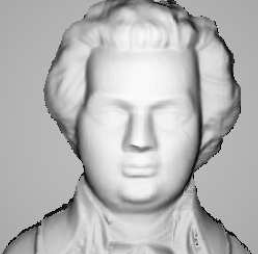
\includegraphics[scale=1]{moz.png}
		\caption{Mozart Initial Image}
		\label{fig:2}
	\end{figure}
	
	\noindent
	The experiments were performed on Fortran90 and results are plotted using MATLAB. The stopping condition for steady state was taken as  $\lVert U^{n+1}-U^{n}\rVert_{\infty} = 10^{-15}$.
	\begin{figure}[h!]
		\begin{subfigure}{0.5\textwidth}
			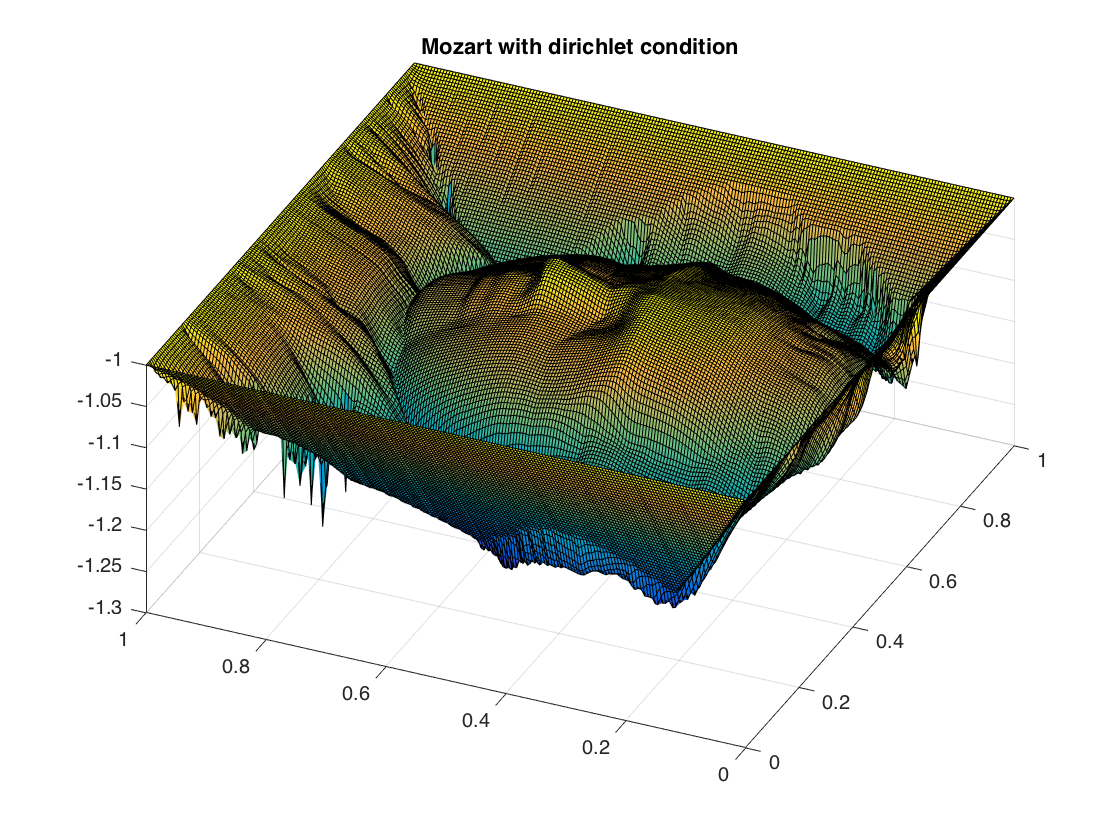
\includegraphics[width = 8cm, height = 7cm]{moz_dirich.png}
			\subcaption{Dirichlet Boundary Condition}
		\end{subfigure}
		~
		\begin{subfigure}{0.5\textwidth}
			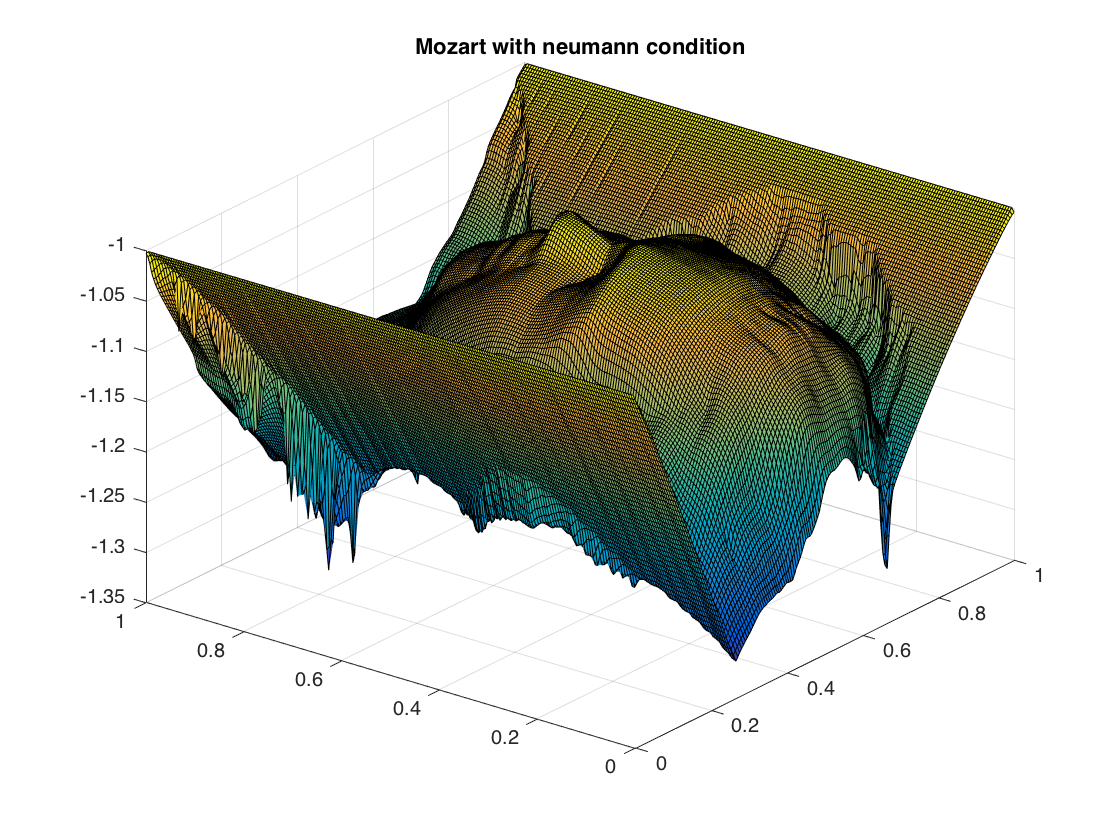
\includegraphics[width = 8cm, height = 7cm]{moz_neu_part.png}
			\subcaption{Neumann Condition on a part of the boundary}			
		\end{subfigure}
		~
		\begin{subfigure}{0.5\textwidth}
			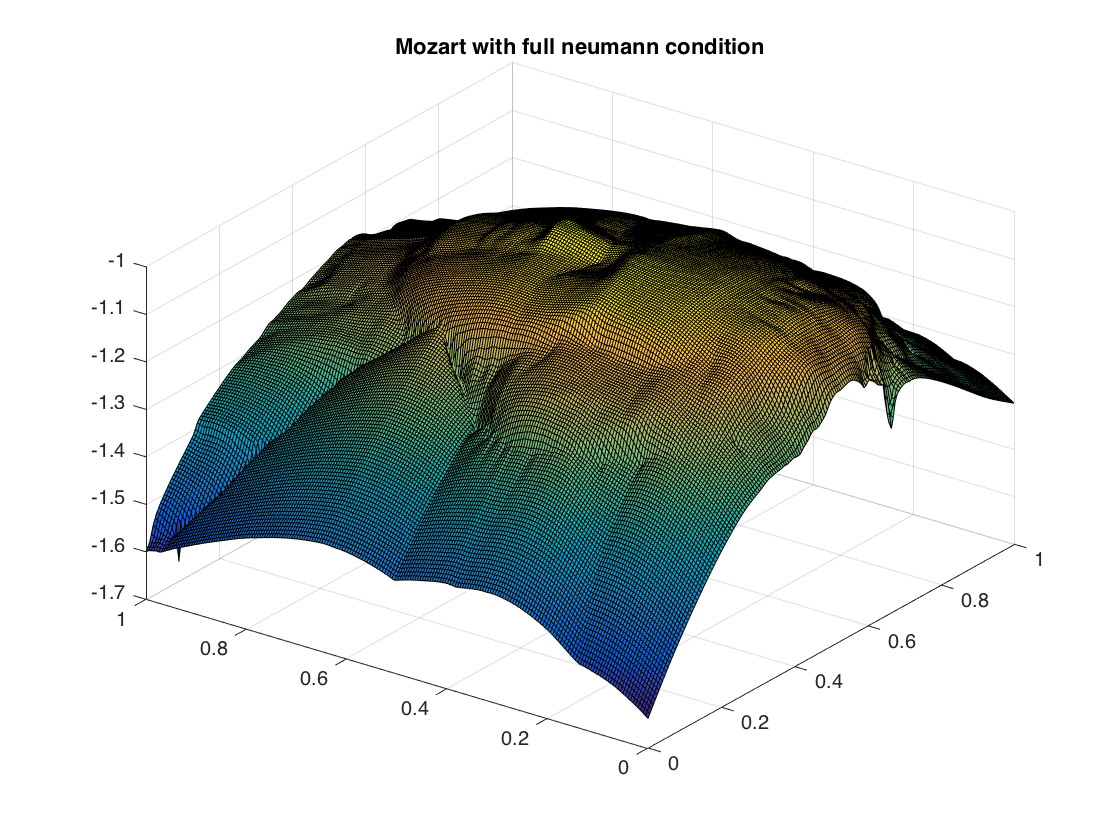
\includegraphics[width = 8cm, height = 7cm]{moz_fneu.png}
			\subcaption{Neumann Condition fully on the boundary}			
		\end{subfigure}
		\caption{Reconstructed Mozart Face}
		\label{fig:3}
	\end{figure}
	
	\noindent
	\subsection{Modification}
	The scheme developed in the previous section can be modified to reduce the oscillations that are present near the boundaries of the reconstructed image. \\
	
	\noindent 
	The idea is to somehow include the Intensity function $I(x,y)$ into the upwinding (\ref{eq:8}) and (\ref{eq:9}). This can be done by taking $I(x,y)$ inside the square root as follows.
	\begin{equation}
		\sqrt{I(\vec{x})^2f^2|\nabla v|^2 + (I(\vec{x})\nabla v. \vec{x})^2 + \frac{I(\vec{x})^2f^2}{|\vec{x}|^2+f^2}} - \frac{f}{\sqrt{|\vec{x}|^2+f^2}} = 0\label{eq:12}
	\end{equation}
	Then the first term $I(\vec{x})^2|\nabla v|^2$ can be upwinded by including the intensity function along with the derivative. 
	\begin{eqnarray}
	\frac{\partial v }{\partial x} &=& \hat{v}_x := \max \left\{ I(x_{i-1},y_j)D_x^-,-I(x_{i+1},y_j)D_x^+,0  \right\}\label{eq:13} \\
	\frac{\partial v }{\partial y} &=& \hat{v}_y := \max \left\{ I(x_i,y_{j-1})D_y^-,-I(x_i,y_{j+1})D_y^+,0  \right\} \label{eq:14}
	\end{eqnarray}
	The $I(x,y)$ in the other terms are kept as it is. This modification reduces the oscillations present near the boundaries of our reconstructed image. The results for the same are shown in Figure (\ref{fig:4}), (\ref{fig:5}) and (\ref{fig:6}).\\
	
	
	\begin{figure}
		\centering
		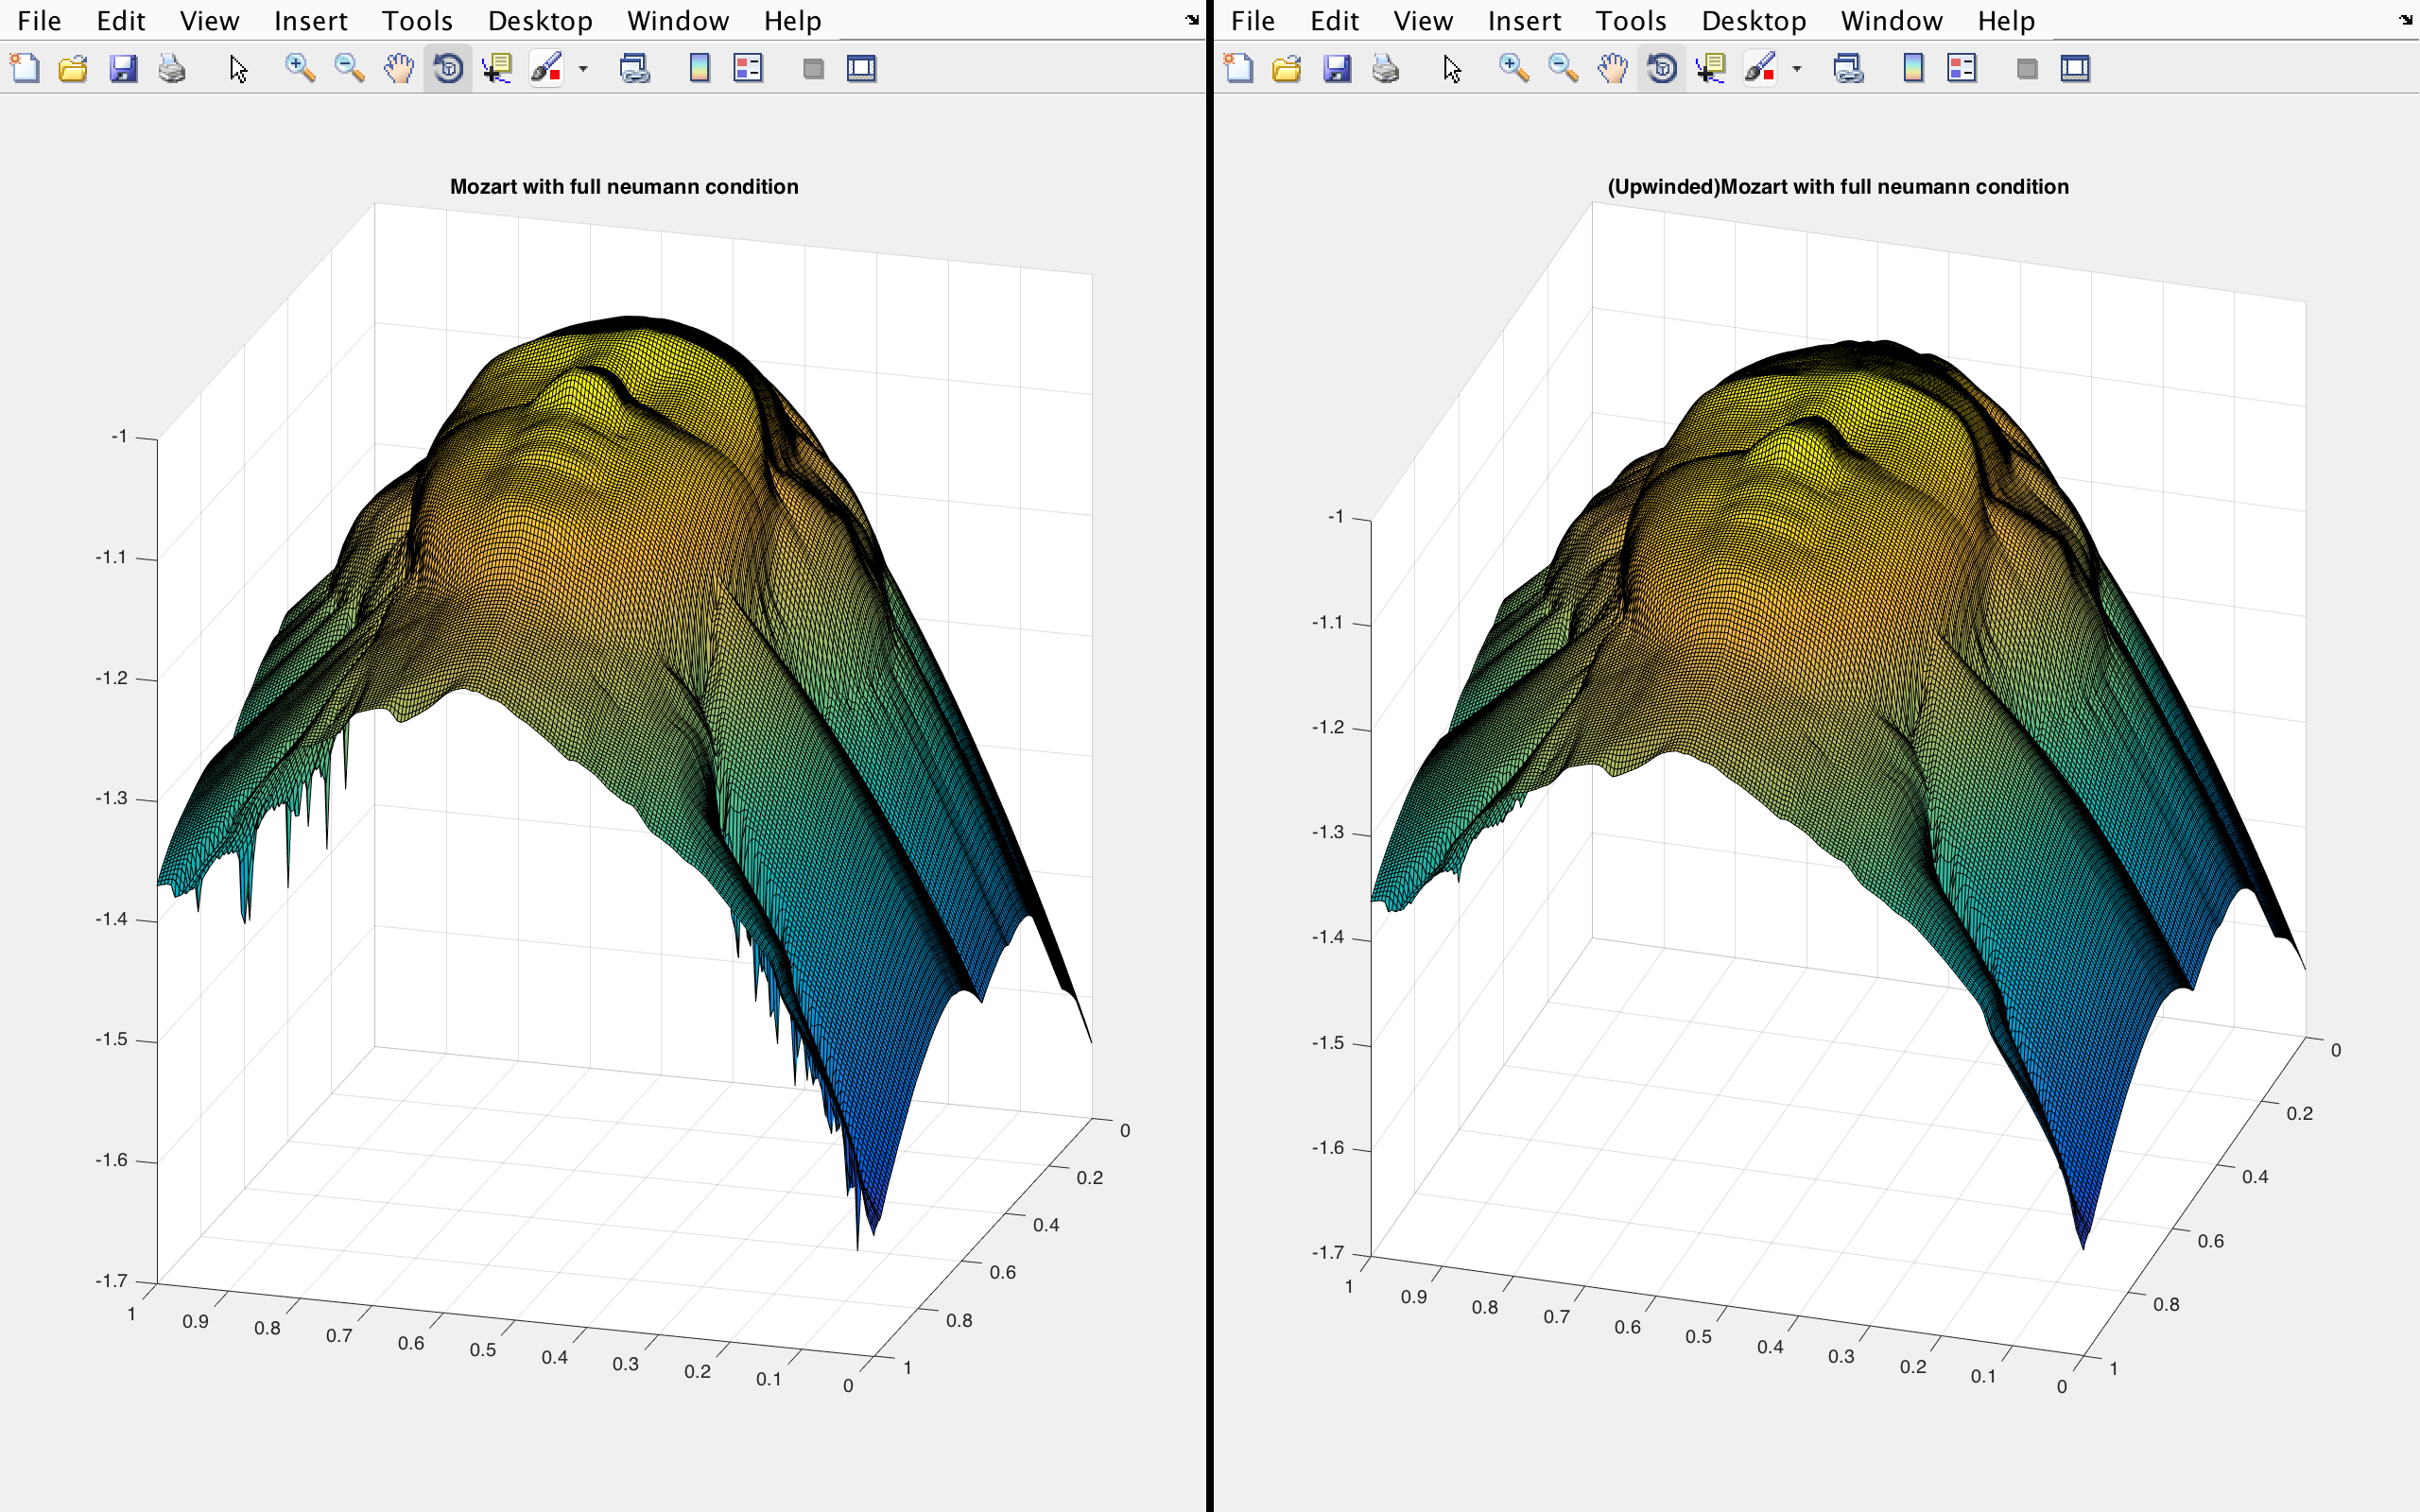
\includegraphics[width = 14cm, height = 7cm]{Compare.png}
		\caption{\textbf{Left} : Without Upwinding  $\;\;\;\;\;\;$ \textbf{Right} : With upwinding}
		\label{fig:4}
	\end{figure}
	 
	\begin{figure}[h!]
		\centering
			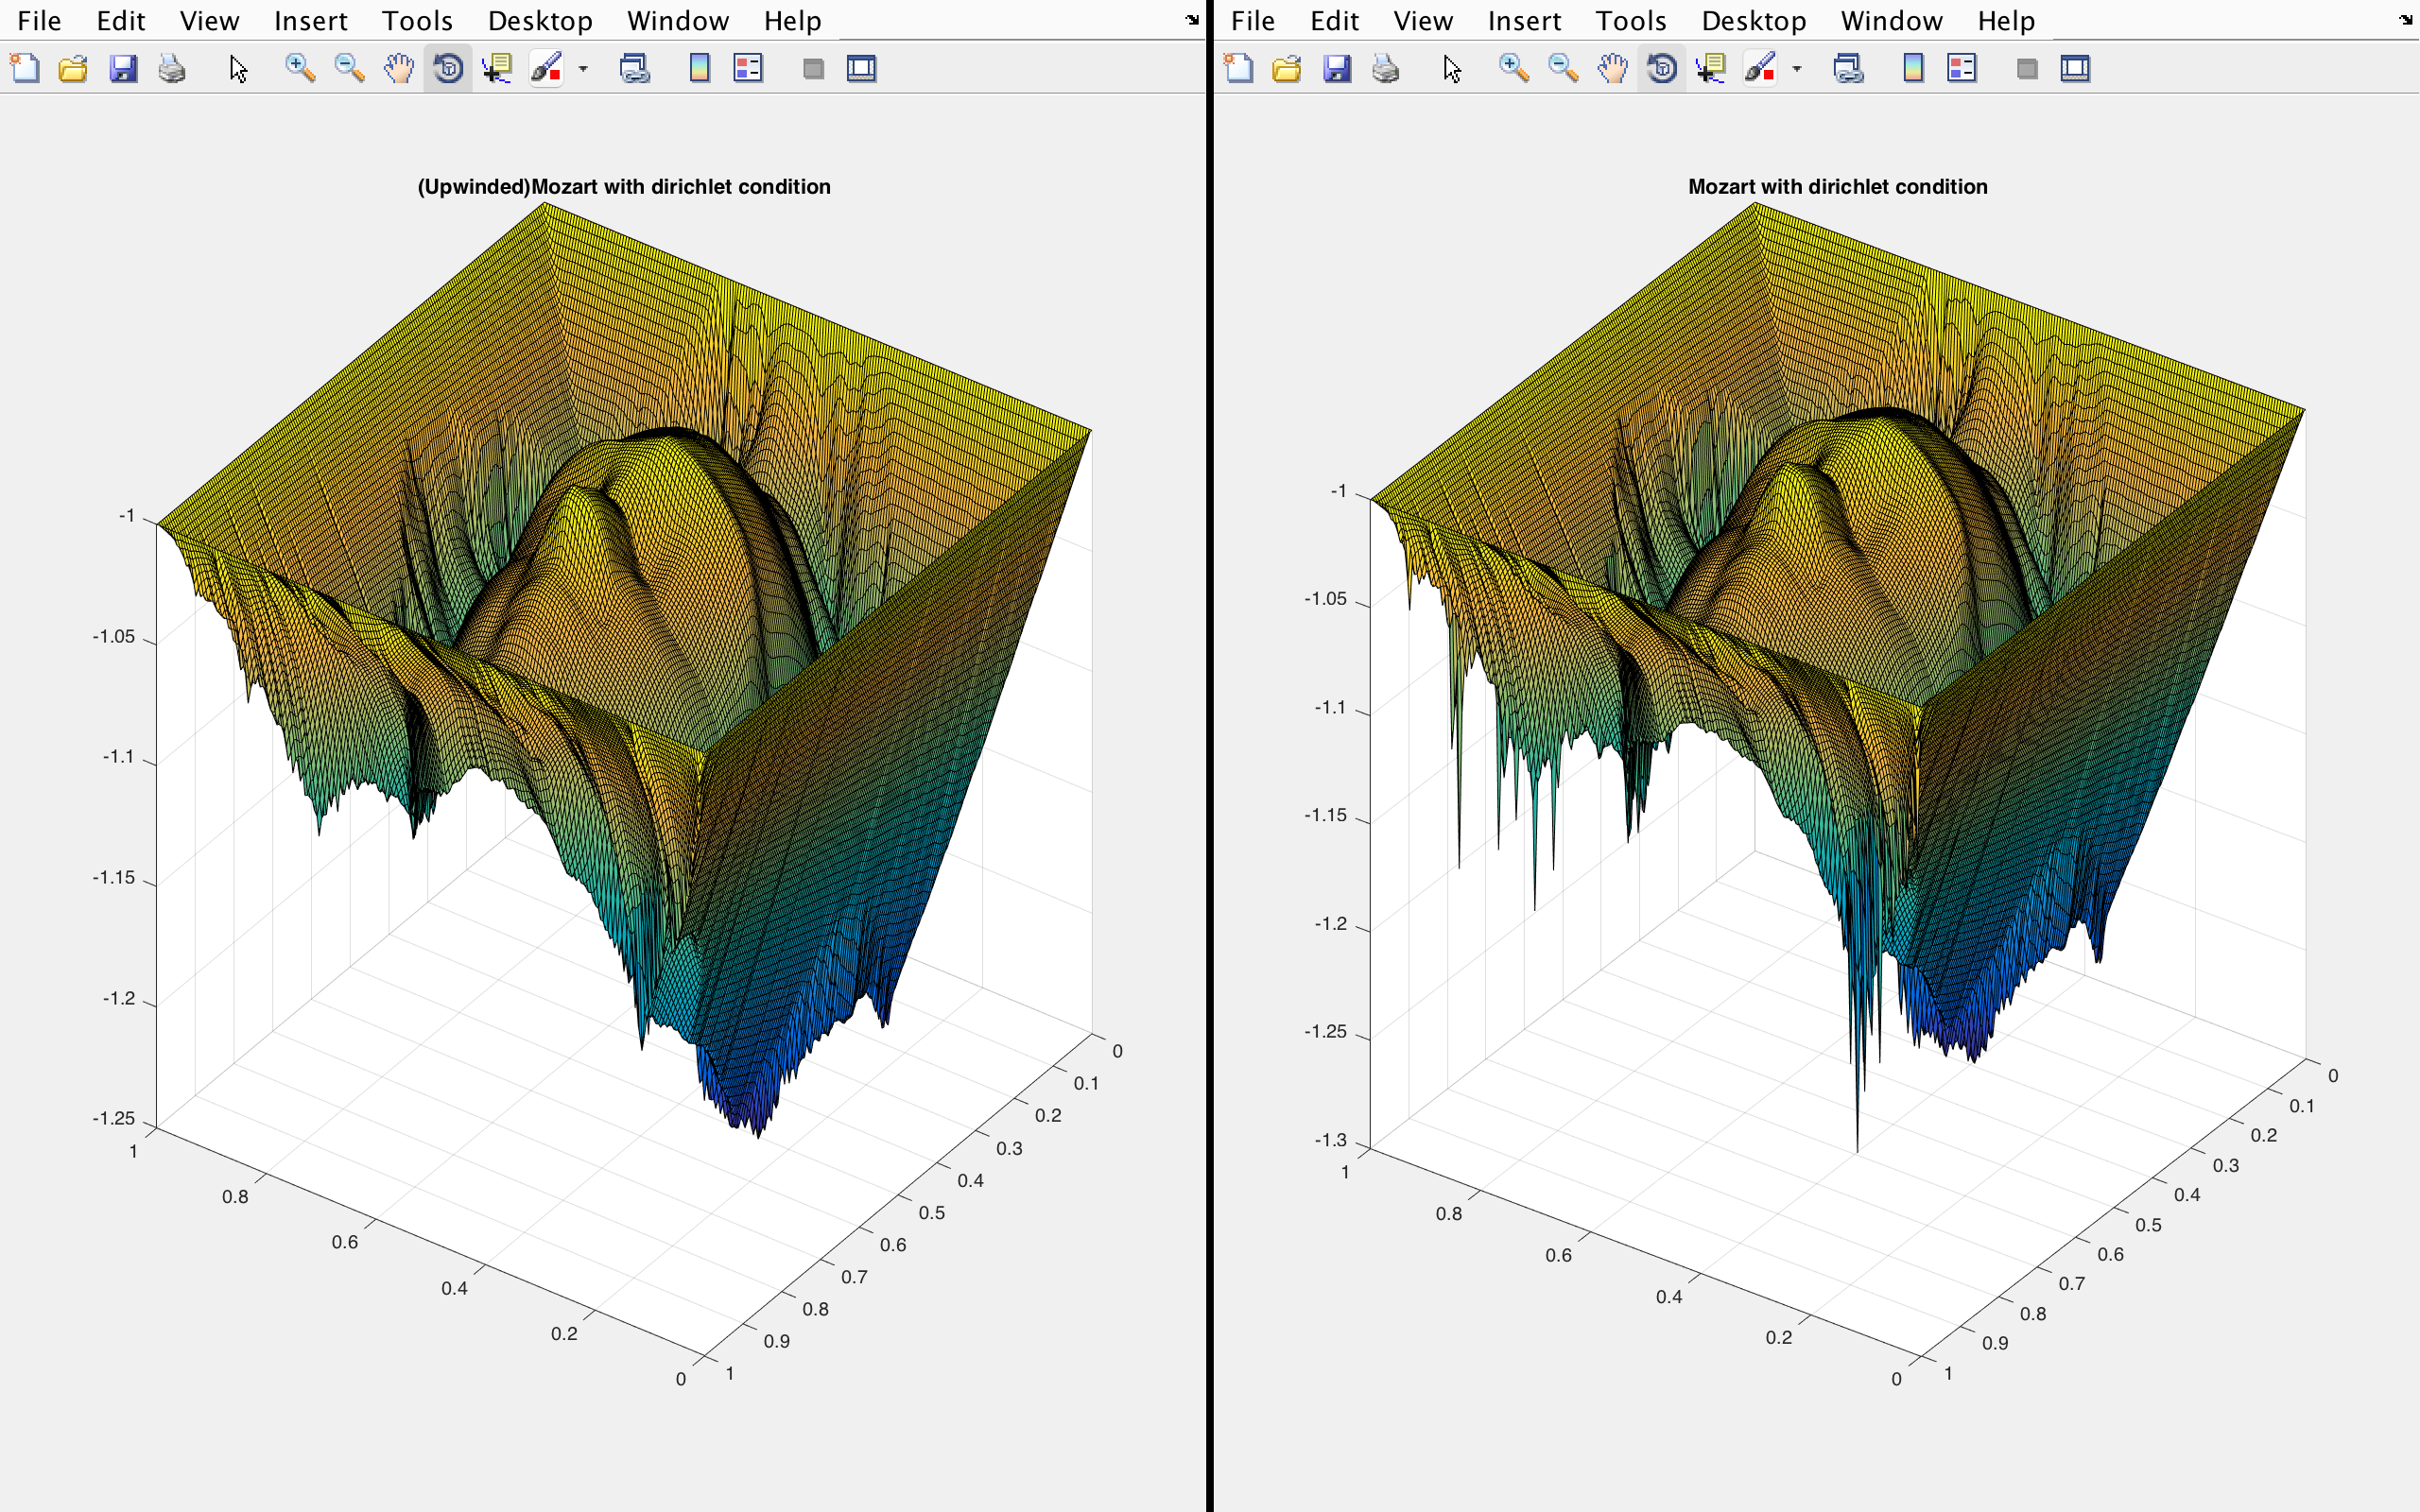
\includegraphics[width = 14cm, height = 7cm]{Compare_dir.png}
			\caption{\textbf{Left} : With Upwinding $\;\;\;\;\;\;$ \textbf{Right} : Without upwinding}
			\label{fig:5}
	\end{figure}
	
		\begin{figure}[h!]
			\centering
			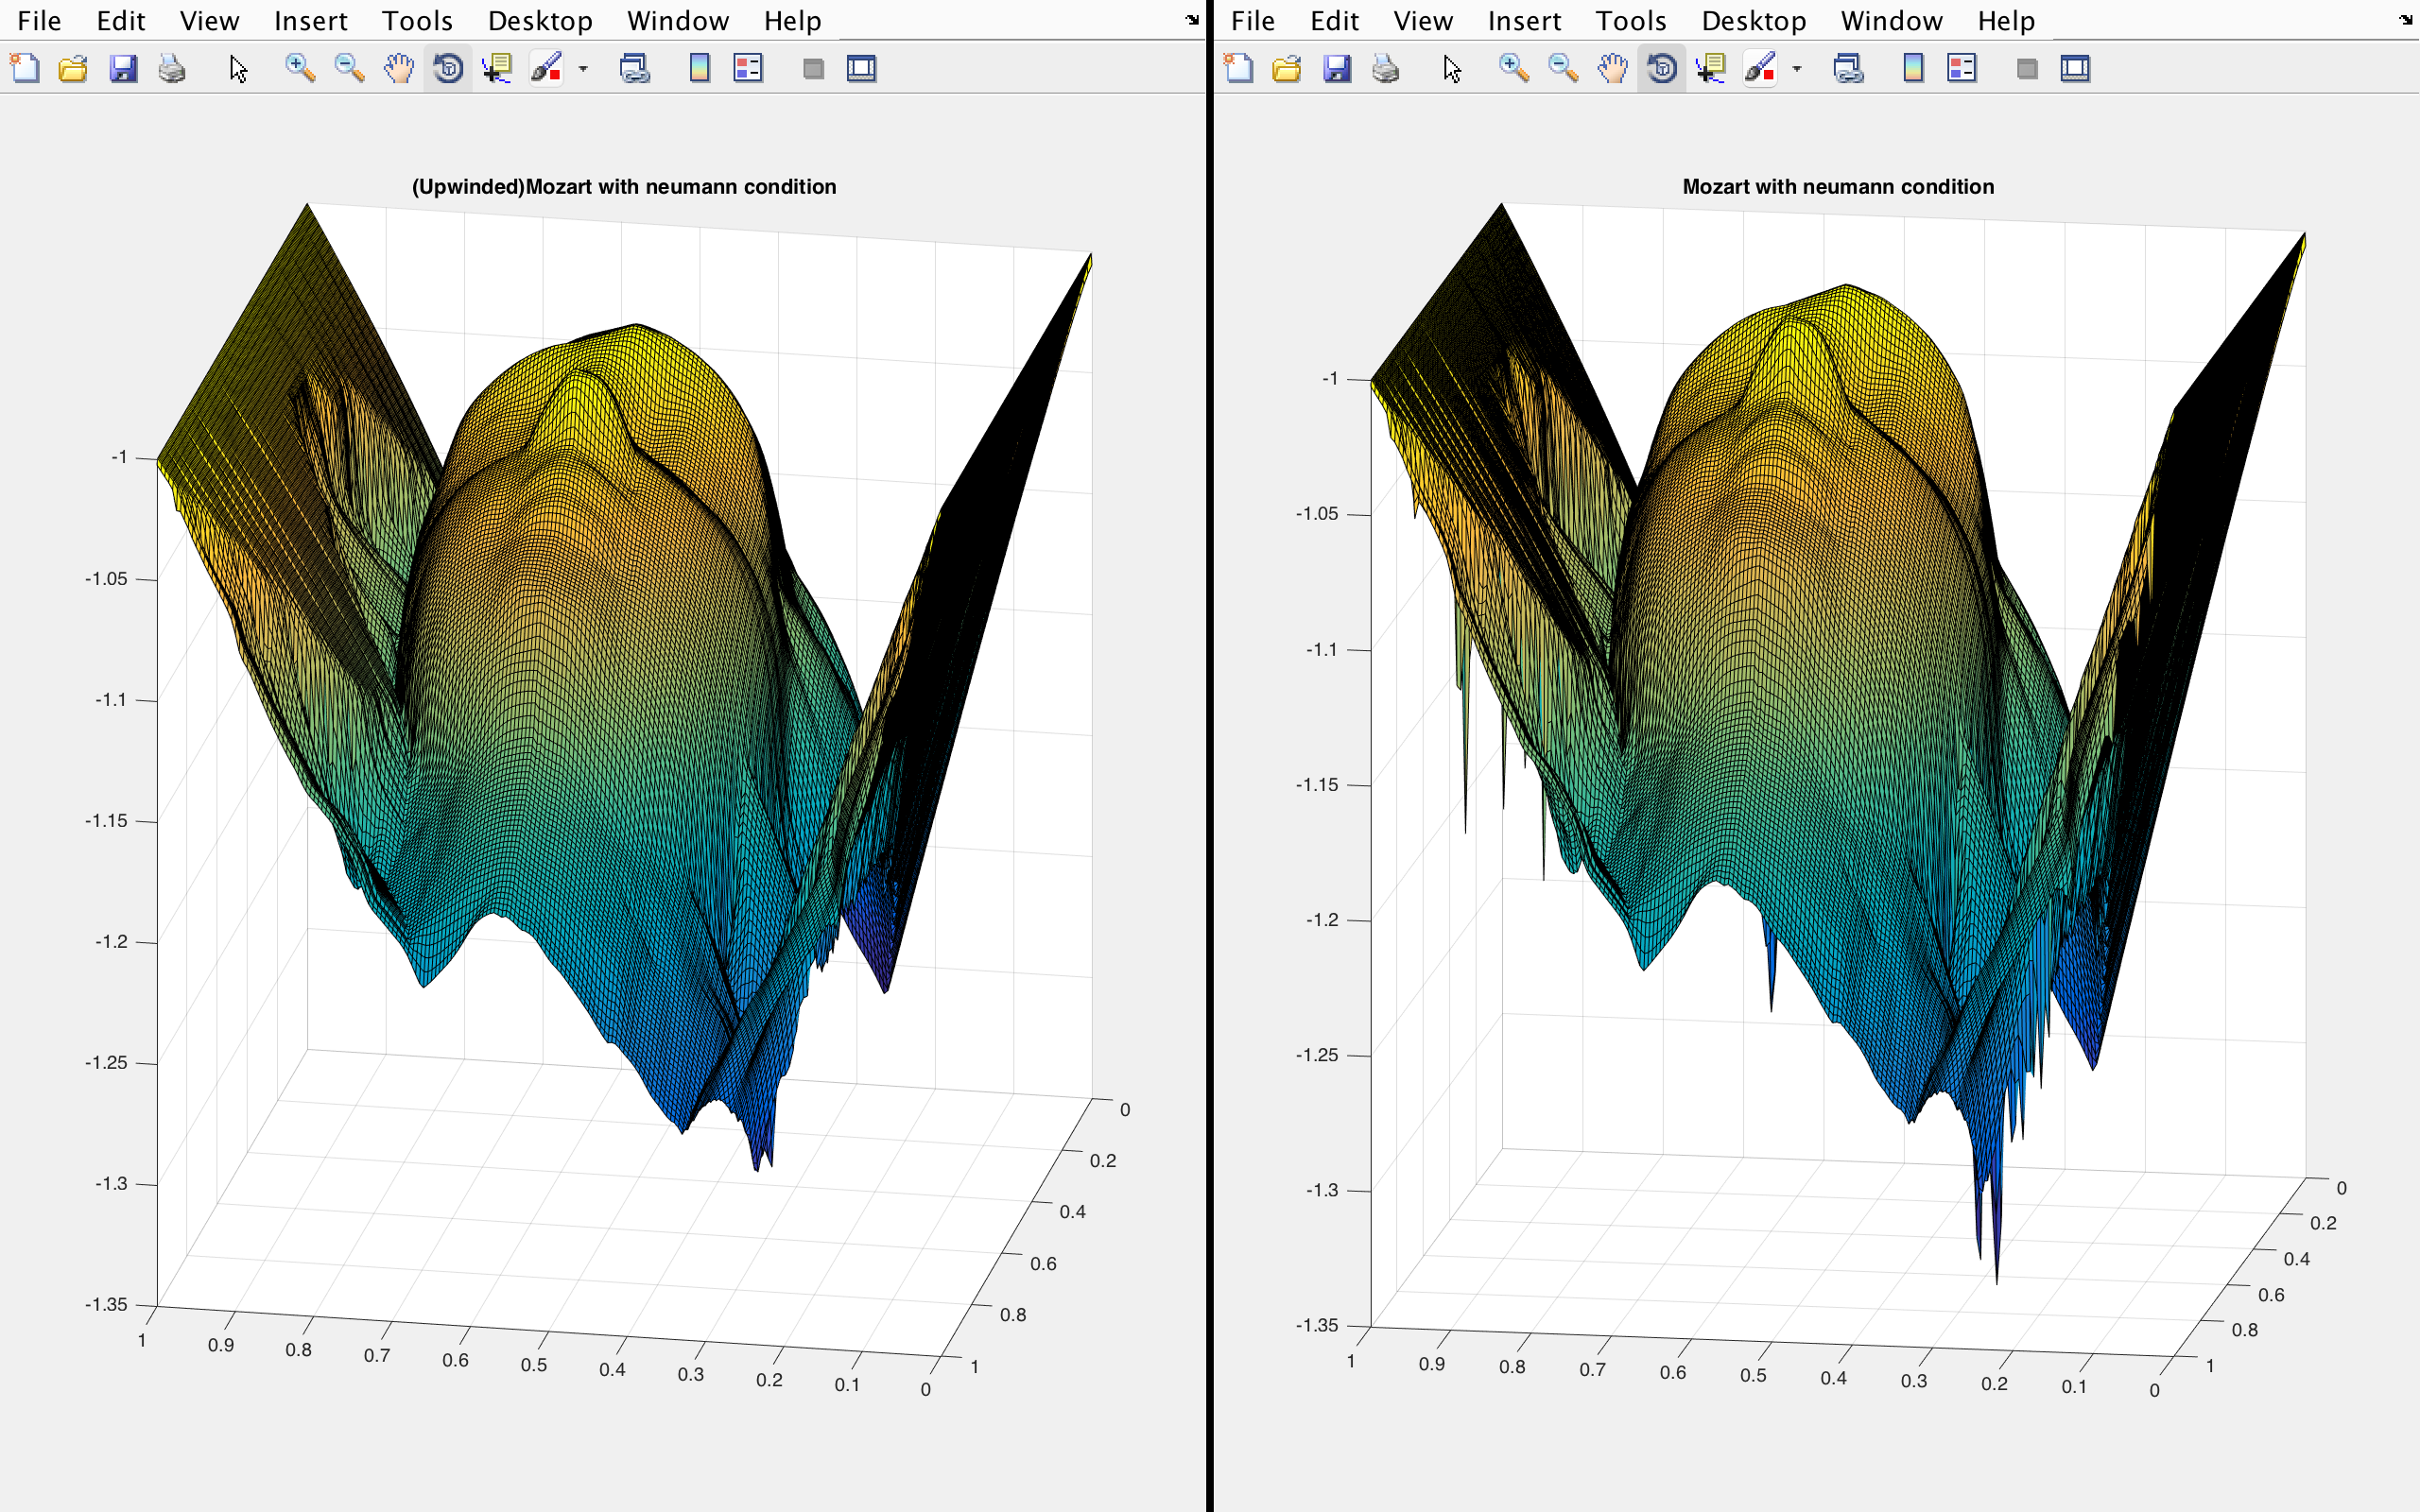
\includegraphics[width = 14cm, height = 7cm]{comapre_newm.png}
			\caption{\textbf{Left} : With Upwinding $\;\;\;\;\;\;$ \textbf{Right} : Without upwinding}
			\label{fig:6}
		\end{figure}
	
	
\end{document}